\documentclass[a4paper, 12pt]{article}
\usepackage{temp}
\usepackage{epsfig,graphicx,subfigure,amsthm,amsmath, float, xcolor, changepage, mathtools, textcomp, hyperref, bm, amssymb, tcolorbox, tikz, setspace}
\usepackage{array}
\usepackage[shortlabels]{enumitem}
\usepackage[bottom]{footmisc}
\usepackage{xepersian}
\settextfont[Scale=1]{XBZar}
%\setdigitfont{XBZar}
\setlatintextfont[Scale=0.9]{Times New Roman}
\hypersetup{
	colorlinks=true,
	urlcolor=blue!70!black
}

\newcolumntype{?}{!{\vrule width 1pt}}

\doublespacing
\begin{document}
	\handout
	{هوش مصنوعی}
	{نیم‌سال اول
		۱۴۰۱\lr{-}۱۴۰۰}
	{دکتر محمدحسین رهبان}
	{دانشکده مهندسی کامپیوتر}
	{مینی‌پروژه پنچم - تئوری}
	{محمدجواد هزاره}
{98101074}
\noindent
\\[-6em]
\section*{سوال ۱}
\begin{enumerate}[A)]
	\item[الف)]
	برای یک استیت مشخص مانند $s$ یکی از مقدایر
	$B_kv_1(s)$
	یا
	$B_kv_2(s)$
	بزرگ‌تر مساوی دیگری است. فرض کنیم این مقدار
	$B_kv_1(s)$
	باشد، بنابراین می‌توان نوشت
	$B_kv_1(s) - B_kv_2(s) \ge 0$.
	حال فرض کنیم اکشن بهینه برای استیت $s$ اکشن $a^\ast$ باشد. بنابراین:
	\[
	B_kv_1(s) = R(s,a^\ast) + \gamma_k \sum_{s^\prime\in\mathcal{S}} p(s^\prime|s, a^\ast) v_1(s^\prime)
	\]
	بنابراین داریم:
	\[
	B_kv_2(s) = \max_a \left[R(s,a) + \gamma_k\sum_{s^\prime\in\mathcal{S}}p(s^\prime|s, a) v_2(s^\prime)\right] \ge \left[R(s,a^\ast) + \gamma_k\sum_{s^\prime\in\mathcal{S}}p(s^\prime|s,a^\ast) v_2(s^\prime)\right]
	\]
	چرا که بیشنه‌ی یک تابع حداقل به‌اندازه‌ی مقدار آن در نقطه‌ای دلخواه است. بنابراین:
	\[
	\dfrac{
		\begin{aligned}
			B_kv_1(s) &= R(s,a^\ast) + \gamma_k \sum_{s^\prime\in\mathcal{S}} p(s^\prime|s, a^\ast) v_1(s^\prime) \\[0.3em]
			-B_kv_2(s) &\le -\left[R(s,a^\ast) + \gamma_k\sum_{s^\prime\in\mathcal{S}}p(s^\prime|s,a^\ast) v_2(s^\prime)\right] \\[0.3em]
		\end{aligned}
	}{\begin{gathered}
		B_kv_1(s) - B_kv_2(s) \le \gamma_k\sum_{s^\prime\in\mathcal{S}}p(s^\prime|s,a^\ast) \left(v_1(s^\prime)-v_2(s^\prime)\right)
	\end{gathered}
	}
	\]
	سمت راست میانگین وزن‌دار تعدادی عبارت است که می‌دانیم این میانگین از قدرمطلق بیشینه‌ی آن‌ها کم‌تر خواهد بود. بنابراین:
	\[
	B_kv_1(s) - B_kv_2(s) \le \gamma_k\sum_{s^\prime\in\mathcal{S}}p(s^\prime|s,a^\ast) \left(v_1(s^\prime)-v_2(s^\prime)\right) \le \gamma_k \|v_1-v_2\|_\infty
	\]
	از طرفی این رابطه برای تمام $s$ها برقرار است، پس برای $s$ای که سمت چپ را بیشینه کند نیز برقرار خواهد بود. هم‌چنین با توجه به آن‌چه در بند اول گفته شد این مقدار مثبت خواهد بود. (اگر مثبت نباشد ممکن بود عدد منفی بزرگی باشد که قدرمطلق آن از سمت راست بیش‌تر می‌شود.) بنابراین:
	\[
	\left.\begin{aligned}
		&\max_s \big(B_kv_1(s) - B_kv_2(s)\big) \le \gamma_k\|v_1-v_2\|_\infty \\
		&0 \le \max_s B_kv_1(s) - B_kv_2(s)
	\end{aligned}\right\}\implies \|B_kv_1-B_kv_2\|_\infty \le \gamma_k\|v_1-v_2\|_\infty
	\]
	در انتخاب $v_1$ و $v_2$ فرض خاصی نکرده بودیم پس استدلال بالا برای تمام هر $v_1$ و $v_2$ برقرار است.
	\item[ب)]
	با جایگذاری
	$\gamma_k = \frac{k}{k+1}$
	خواهیم داشت:
	\[
	\prod_{k=1}^{K}\gamma_k = \frac{1}{2}\times\frac{2}{3}\times\cdots\times\frac{K-1}{K}\times\frac{K}{K+1} = \frac{1}{K+1} \le \frac{1}{K+1}
	\]
	\item[ج)]
	اگر برای دو بردار $v_1$ و $v_2$ به ترتیب $K$ مرحله عملگر $B_k$ را اعمال کنیم، با توجه به انقباضی بودن تمام $B_k$ها خواهیم داشت:
	\[
	\begin{aligned}
		0\le\|B_K\cdots B_1v_1 - B_K\cdots B_1v_2\|_\infty &\le \gamma_K\|B_{K-1}\cdots B_1v_1 - B_{K-1}\cdots B_1v_2\|_\infty \\[0.3em]
		&\le\gamma_K\gamma_{K-1}\|B_{K-2}\cdots B_1v_1 - B_{K-2}\cdots B_1v_2\|_\infty \\[0.3em]
		&\le\qquad\vdots \\
		&\le\gamma_K\cdots\gamma_1 \|v_1 - v_2\|_\infty \\[0.3em]
		&\le\frac{1}{1+K}\|v_1 - v_2\|_\infty
	\end{aligned}
	\]
	هم‌چنین برای بردار
	$\overrightarrow 0$
	داریم:
	\[
	B_K\cdots B_1\overrightarrow{0} = \gamma_KR_K + \gamma_K\gamma_{K-1}R_{K-1} + \cdots + \gamma_1R_1 + R_0
	\]
	که اگر مقدار پاداش‌ها متناهی باشد، با $K\to\infty$ عبارت بالا به مقداری متناهی هم‌گرا شده که آن را با $v^\ast$ نشان می‌دهیم که این مقدار همان مطلوبیت استیت‌ها خواهد بود. حال اگر در رابطه‌ی بالا بردار $v_2$ را همان بردار
	$\overrightarrow 0$
	در نظر بگیریم، در حد $K\to\infty$ خواهیم داشت:
	\[
	\begin{gathered}
		\left.\begin{gathered}
			0 \le \lim_{K\to\infty} \|B_K\cdots B_1v_1 - v^\ast\|_\infty \\[0.3em]
			\lim_{K\to\infty} \|B_K\cdots B_1v_1 - v^\ast\|_\infty \le \lim_{K\to\infty} \frac{1}{1+K}\|v_1 - \overrightarrow 0\|_\infty = 0
		\end{gathered}\right\}\implies \lim_{K\to\infty}\|B_K\cdots B_1v_1 - v^\ast\|_\infty = 0 \\[2.5em]
	\implies \lim_{K\to\infty} B_K\cdots B_1v_1 = v^\ast
	\end{gathered}
	\]
	که در استدلال بالا فرض خاصی برای $v_1$ نکردیم، بنابراین استدلال برای هر $v_1$ای برقرار است.
	\item[د)]
	به مقدار $\gamma$ در روش ضریب ثابت بستگی دارد. اگر $\gamma$ به‌اندازه‌ی کافی کوچک باشد روش ضریب ثابت بهتر عمل می‌کند و سریع‌تر به نزدیکی صفر می‌رسد. اما اگر $\gamma$ به‌اندازه‌ی کافی بزرگ باشد استفاده کردن از روش جدید مناسب‌تر است چرا که سریع‌تر به صفر نزدیک می‌شود. به نمودارهای زیر می‌توان دقت کرد.
	\begin{figure}[H]
		\centering
		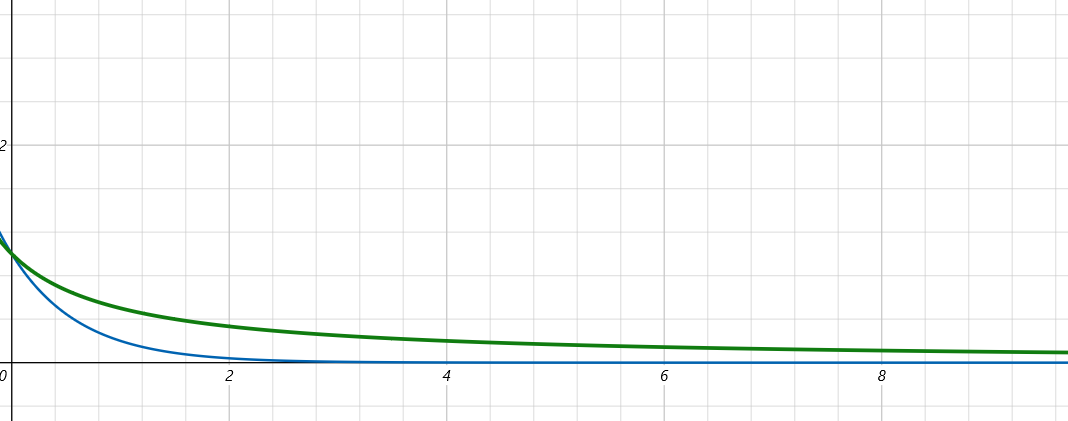
\includegraphics[width=0.45\textwidth]{constant.png}
		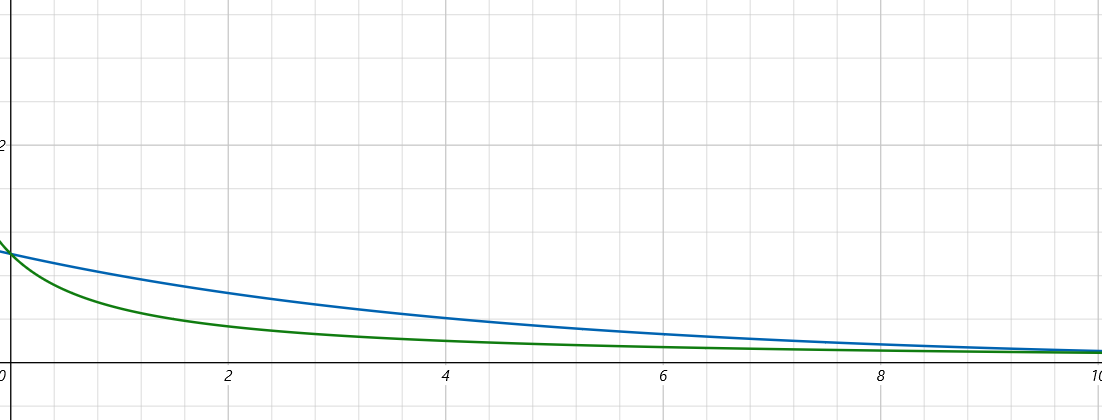
\includegraphics[width=0.45\textwidth]{new.png}
		\caption{
			{\scriptsize
		نمودار آبی مربوط به روش ضریب ثابت و نمودار سبز مربوط به روش ضریب متغیر است. (در سمت راستی $\gamma=0.2$ و در سمت چپی $\gamma=0.8$)	
		}
		}
	\end{figure}
\end{enumerate}

\pagebreak
\section*{سوال ۲}
\begin{enumerate}
	\item[الف)]
	با توجه به تصادفی بودن سیاست داده شده، برای محاسبه‌ی $v_\Pi$ باید احتمال انجام شدن یک اکشن را در $Q$ آن ضرب کرده و روی اکشن‌های مختلف جمع ببندیم. بنابراین:
	\[
	v_\Pi(s) = \sum_{a} \Pi_{s,a} Q(s,a)
	\]
	برای محاسبه‌ی $Q$ نیز باید روی استیت‌های مختلف جمع بزنیم:
	\[
	\begin{aligned}
		Q(s, a) &= \sum_{s^\prime} p(s^\prime|s, a)\left[W_{s,s^\prime} + \gamma v_\Pi(s^\prime)\right] \\[0.4em]
		&= \eta \big[W_{s,a} + \gamma v_\Pi(a)\big] + \frac{1-\eta}{d_s}\sum_{i\in N(s)} \big[W_{s,i} + \gamma v_\Pi(i)\big]
	\end{aligned}
	\]
	که $N(s)$ همسایه‌های $s$ هستند. بنابراین برای $v_\Pi$ می‌توان نوشت:
	\[
	v_\Pi(s) = \sum_a \Pi_{s,a} \left[\big[W_{s,a} + \gamma v_\Pi(a)\big] + \frac{1-\eta}{d_s}\sum_{i\in N(s)} \big[W_{s,i} + \gamma v_\Pi(i)\big]\right]
	\]
	برای محاسبه‌ی $v^\ast$ بهتر است از تصمیمات قطعی استفاده کنیم چرا که بیشنه‌ی $Q$ها از هر میانگین وزن‌دار آن‌ها بیش‌تر خواهد بود. بنابراین در یک استیت $s$ بهتر است به استیتی برویم که $Q(s,a)$ را بیشینه می‌کند. بنابراین روی اکشن‌های مختلفی که از $s$ می‌توان انجام داد بیشینه می‌گیریم:
	\[
	v^\ast(s) = \max_a \left[\big[W_{s,a} + \gamma v^\ast(a)\big] + \frac{1-\eta}{d_s}\sum_{i\in N(s)} \big[W_{s,i} + \gamma v^\ast(i)\big]\right]
	\]
	\item[ب)]
	اگر $\eta = 1$ باشد داریم:
	\[
	v_\Pi(s) = \sum_{a} \Pi_{s,a}\big[W_{s,a} + \gamma v_\Pi(a)\big] = \sum_{a}  \Pi_{s,a} W_{s,a} + \gamma\sum_{a}\Pi_{s,a}v_\Pi(a)
	\]
	جمله‌ی دوم به شکل برداری برابر
	$\gamma \Pi v_\Pi$
	خواهد بود. جمله‌ی اول نیز به‌ازای یک $s$ مشخص، جمع سطر $s$ام از ماتریس
	$\Pi \odot W$
	خواهد بود، بنابراین به شکل ماتریسی به فرم 
	$(\Pi \odot W)\overrightarrow{1}$
	خواهد بود. بنابراین برای رابطه‌ی بلمن به شکل ماتریسی داریم:
	\[
	\begin{gathered}
		v_\Pi = \gamma \Pi v_\Pi + (\Pi \odot W)\overrightarrow{1} \\[0.4em]
		\implies \boxed{[I - \gamma \Pi]v_\Pi = (\Pi \odot W)\overrightarrow{1}}
	\end{gathered}
	\]
	\item[ج)]
	با توجه به قسمت قبل می‌توان نوشت:
	\[
	v_\Pi = [I - \gamma \Pi]^{-1}(\Pi \odot W)\overrightarrow{1}
	\]
	اما برای پیدا کردن بهترین سیاست باید $\Pi$ را به‌گونه‌ای انتخاب کنیم که تک تک درایه‌های $v_\Pi$ بیش‌ترین مقدار خود را داشته باشند. از طرفی مشخصا نمی‌خواهیم در سیاست خود برای رفتن از راس $i$ به راس $j$ که یالی به یکدیگر ندارند احتمالی در نظر بگیریم. به عبارتی در سیاست ما باید
	$\Pi_{i,j} = 0$
	باشد اگر $i$ به $j$ یالی نداشته باشد. هم‌چنین به‌ازای هر راس مثل $i$، جمع احتمال تصمیم‌هایی که می‌گیریم باید برابر یک شود که این شرط نیز به شکل
	$\Pi\overrightarrow{1} = \overrightarrow{1}$
	ظاهر می‌شود.
\end{enumerate}

\end{document}



